\documentclass[portrait,a0]{a0poster}
\usepackage{fontspec}

\setmainfont{Bai Jamjuree}
\newfontfamily\extrabold{Bai Jamjuree Bold}

\usepackage[framemethod=TikZ]{mdframed}
\usepackage{lipsum}
\usepackage{graphicx}
\usepackage{setspace}

\usepackage[margin=3cm,nomarginpar]{geometry}
\usepackage{multicol}

\definecolor{ciblue}{RGB}{1, 30, 66}
\definecolor{ciyellow}{RGB}{255, 199, 44}

\mdfdefinestyle{mainbox}{
    innerleftmargin=1cm,innerrightmargin=1cm,
    roundcorner=5mm,
    linewidth=1mm,
    linecolor=ciblue
}

\mdfdefinestyle{highlightbox}{
    innerleftmargin=1cm,innerrightmargin=1cm,
    roundcorner=5mm,
    linewidth=1mm,
    linecolor=ciyellow,
    backgroundcolor=ciyellow!50!white
}

\mdfdefinestyle{partners}{
    innerleftmargin=1cm,innerrightmargin=1cm,
    roundcorner=5mm,
    linewidth=0.5mm,
    linecolor=ciblue!20!white
}

\newcommand{\mainbox}[3]{
    \begin{mdframed}[style=mainbox]
        \begin{center}
            \vspace{5mm}
            {\extrabold \Huge #1}
        \end{center}
        \vspace{5mm}
        \parbox[t][#2][t]{\linewidth}{\large
            #3
        }
    \end{mdframed}
}

\begin{document}
\noindent\begin{minipage}[t]{0.3\textwidth}
    \includegraphics[scale=3]{di-osvise}
\end{minipage}
\begin{minipage}[c]{0.7\textwidth}
\begin{flushright}
    \begin{spacing}{1}
        \VERYHuge \extrabold \color{ciblue}Open Source Verification of \\ Instruction Set Extensions%
    \end{spacing}
\end{flushright}
\end{minipage}

\noindent\begin{minipage}[t]{386mm}
    \mainbox{Motivation}{23cm}{
        DI-OSVISE is motivated by the need for open source tools for verfication of instruction set extensions:
        \begin{itemize}
            \item RISC-V enables domain-specific instruction set extensions
            \item Fast evaluation of custom extensions needed
            \item Dynamic and formal verification with open source tools
            \item Impact of non-functional properties
        \end{itemize}
        \vfill
        \begin{mdframed}[style=highlightbox]
            {\extrabold \Large State-of-the-Art}
            \large
            \begin{itemize}
                \item Simulation-based verification of entire CPU (TRL 9), separation of ISA extension experimental (TRL 1)
                \item Validation of non-functional properties of ISA extensions for simple pipelines (TRL 1-2)
                \item CIRCT framework only supports logic, no LTL and lowering (TRL 1)
                \item Proof-of-Concept UVM support in Verilator (TRL 2-3)
            \end{itemize}
        \end{mdframed}
        \vfill
        }
\end{minipage}%
\hfill
\begin{minipage}[t]{386mm}
    \mainbox{Innovation}{23cm}{
        Central to DI-OSVISE: \textbf{Interoperability
        and Readiness} of open source tools for verification of ISA extensions.
        \begin{description}
            \item[Simulation-based Functional Verification of ISA Extensions (AP 2)] \hfill \newline
            $\rightarrow$ High-performance ISS/RTL simulation with automated generation of inter-simulator interfaces from compact abstract descriptions (TRL 4-5)
            $\rightarrow$ Improved UVM support of Verilator, integration in real world open source verification (TRL 4-5)
            \item[Simulation-based Verification of Non-Functional Properties (AP 3)] \hfill \newline
            $\rightarrow$ Open source simulator to validate performance improvement and power corridors for complex pipelines with ISA Extension (TRL 
            4-5)
            \item[End-to-end support for Linear Temporal Logic (AP4)] \hfill \newline
            $\rightarrow$ LTL-IR and the appropriate front ends and exemplary passes enable the development of further tools for (formal) verification based on the LLVM framework CIRCT (TRL 4) \\
            $\rightarrow$ Better interoperability of tools and an exemplary basis for the efficient exploratory evaluation of instruction set extensions (TRL 4-5)
        \end{description}
    }
\end{minipage}

\vspace{9mm}

\noindent\begin{minipage}[t]{\textwidth}
    \mainbox{Project Overview}{30cm}{
    \begin{minipage}{40cm}
        \includegraphics[width=40cm]{overview.drawio}
    \end{minipage}
    \hfill
    \begin{minipage}{30cm}
        DI-OSVISE builds on well-established Open Source EDA tools. Contributions are planned upstream in those projects and we collaborate with project maintainers. Own projects will be released on GitHub under permissive licenses.

        \bigskip

        \begin{mdframed}[style=highlightbox]
            {\extrabold \Large Impact}
            \begin{itemize}
                \item Complete Open Source toolchain for functional verification of RISC-V based microprocessors
                \item Open Source tool for fast exploration of ISA extensions with combined ISS/RTL simulation
                \item Open Source simulator for validation of performance improvements and power corridors
                \item Improved usability of CIRCT with (System)Verilog, especially assertions, and PSL support
                \item LTL-IR as CIRCT dialect as enablement for more open source EDA tools around (formal) verification
                \item Yosys verification flow usable without proprietary license
                \item core-v-verif and similar verification flows without proprietary license
            \end{itemize}
        \end{mdframed}

        \end{minipage}
    }
\end{minipage}

\vspace{9mm}

\noindent\begin{minipage}[t]{\textwidth}
    \mainbox{Roadmap}{9cm}{
        \centering
    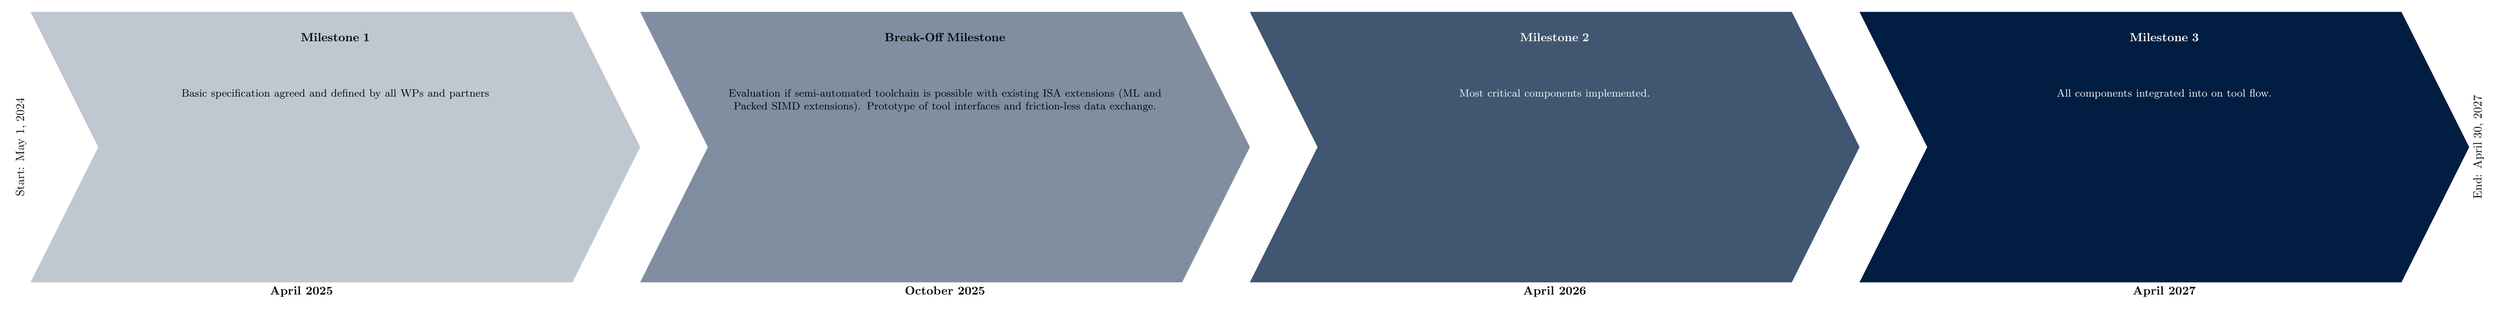
\begin{tikzpicture}
        \node [anchor=south,rotate=90] at (0,4) {Start: May 1, 2024};
        \fill[ciblue!25!white] (0,0) -- (2,4) -- (0,8) -- (16,8) -- (18,4) -- (16,0) -- cycle;
        \node [anchor=north,text width=14cm,align=center] at (9,7.5) {\textbf{Milestone 1}};
        \node [anchor=north,text width=14cm,align=center] at (9,6) {\begin{spacing}{1}\small Basic specification agreed and defined by all WPs and partners\end{spacing}};
        \node [anchor=north] at (8,0) {\textbf{April 2025}};
        \fill[ciblue!50!white] (18,0) -- (20,4) -- (18,8) -- (34,8) -- (36,4) -- (34,0) -- cycle;
        \node [anchor=north,text width=14cm,align=center] at (27,7.5) {\textbf{Break-Off Milestone}};
        \node [anchor=north,text width=14cm,align=center] at (27,6) {\begin{spacing}{1}\small Evaluation if semi-automated toolchain is possible with existing ISA extensions (ML and Packed SIMD extensions). Prototype of tool interfaces and friction-less data exchange.\end{spacing}};
        \node [anchor=north] at (27,0) {\textbf{October 2025}};
        \fill[ciblue!75!white] (36,0) -- (38,4) -- (36,8) -- (52,8) -- (54,4) -- (52,0) -- cycle;
        \node [anchor=north,text width=14cm,align=center] at (45,7.5) {\color{white}\textbf{Milestone 2}};
        \node [anchor=north,text width=14cm,align=center] at (45,6) {\begin{spacing}{1}\color{white}\small Most critical components implemented.\end{spacing}};
        \node [anchor=north] at (45,0) {\textbf{April 2026}};
        \fill[ciblue] (54,0) -- (56,4) -- (54,8) -- (70,8) -- (72,4) -- (70,0) -- cycle;
        \node [anchor=north,text width=14cm,align=center] at (63,7.5) {\color{white}\textbf{Milestone 3}};
        \node [anchor=north,text width=14cm,align=center] at (63,6) {\begin{spacing}{1}\color{white}\small All components integrated into on tool flow.\end{spacing}};
        \node [anchor=north] at (63,0) {\textbf{April 2027}};
        \node [anchor=north,rotate=90] at (72,4) {End: April 30, 2027};
    \end{tikzpicture}
}
\end{minipage}

\vspace{9mm}

\noindent\begin{minipage}[t]{500mm}
    \mainbox{Partners}{17cm}{
    \hfill
    \begin{minipage}{0.5\textwidth}
        \begin{mdframed}[style=partners]
            \parbox[t][13cm][t]{\linewidth}{
                \begin{tikzpicture}
                    \node at (0,0) {\includegraphics[height=3.5cm]{YOS_horiz}};
                    \node at (6,0) {\includegraphics[height=4cm]{planv}};
                    \node at (12,0) {\includegraphics[height=1.7cm]{Minres_logo}};
                    \node at (1,-4) {\includegraphics[height=3cm]{HM_Schriftzug_Logo_rot_RGB}};
                    \node at (12,-4) {\includegraphics[height=2.8cm]{TU_Muenchen_Logo}};
                    \node at (-1,-8) {\includegraphics[height=3cm]{TU_Darmstadt_Logo}};
                    \node at (6,-8) {\includegraphics[height=2cm]{TU_Wien-Logo}};
                    \node at (13.5,-8) {\includegraphics[height=3.5cm]{Logo_Uni_Luebeck_CMYK}};
                \end{tikzpicture}
            }
        \end{mdframed}
        \centering
        Funded Partners
    \end{minipage}
    \hfill
    \begin{minipage}{0.4\textwidth}
        \begin{mdframed}[style=partners]
            \parbox[t][13cm][t]{\linewidth}{
            \centering
            \vfill
            
            \hfill \includegraphics[height=3cm]{Infineon-Logo} \hfill 
            
\includegraphics[height=2cm]{NXP_Semiconductors_logo_2023} \hfill

            \vfill

            \includegraphics[height=2cm]{Qualcomm-Logo}
            \vfill
            \includegraphics[height=3cm]{SiFive_logo}
            \vfill

            }
        \end{mdframed}
        \centering
        Associated Partners
    \end{minipage}
    \hfill
    }
\end{minipage}
%
\hfill
%
\begin{minipage}[t]{272mm}
    \mainbox{Funding Information}{13cm}{
        This project is funded by the German Federal Ministry of Education and Research.
        
        \medskip

        \emph{Funding Amount:} € 1,978,906
        
        \emph{Reference number:} 16ME0953

        \vfill

        \centering
            
            \includegraphics[width=0.6\textwidth]{BMBF_Logo}

    }
    \raggedleft \Large \color{ciblue} \textbf{https://di-osvise.github.io}
\end{minipage}

\end{document}